\documentclass[12pt]{article}

% Set page size and margins
\usepackage[a4paper,top=2cm,bottom=2cm,left=2cm,right=2cm,marginparwidth=1.75cm]{geometry}

% Language setting
\usepackage[english,main=greek]{babel}


% Page background & text colors
\usepackage[dvipsnames]{xcolor}
% define bg and txt colors
\definecolor{col_bg}{HTML}{FFFFFF} 
\definecolor{col_txt}{HTML}{000000}
% set the colors
\pagecolor{col_bg}
\color{col_txt}


% Useful packages
\usepackage{amsmath,amssymb}
\usepackage{amsfonts}
\usepackage[utf8]{inputenc}
\usepackage[T1]{fontenc}
\usepackage{csquotes}
\usepackage{graphicx}
\usepackage{csquotes}
\usepackage{listings}
\usepackage{algorithm}
\usepackage{algpseudocode}
\usepackage{enumitem}
\usepackage{tabularray}
\usepackage{tikz}
\usepackage{colortbl}
\usepackage{bm}

% Create plots
\usepackage{pgfplots}
\pgfplotsset{compat=newest}

% Use: \en{english text}
\newcommand{\en}[1]{\foreignlanguage{english}{#1}}


\begin{document}

\begin{table}[ht]
    \begin{tblr}{
      @{}X[l,valign=b]X[c,valign=b]X[r,valign=b]@{}
    }

        % First line, course info
        \hline
        \SetCell[c=2]{l}{[Κ17] Αλγόριθμοι \& Πολυπλοκότητα} & & {2023-24} \\ 
        \hline
        {} & {} & {} \\

        % Title
        \SetCell[c=3]{c}{ \Large \textbf{Εργασία 0} } \\
        {} & {} & {} \\

        % Info
        \SetCell[c=3]{c}{ \large \it Απαντήσεις  } \\
        {} & {} & {} \\
        
        % Name Surname, RN
        \hline
        \SetCell[c=3]{c}{ \textbf{Ονοματεπώνυμο:} Όνομα Επώνυμο } \\
        \SetCell[c=3]{c}{ \textbf{Α.Μ.:} 1115 \ldots } \\
        \hline
        
    \end{tblr}
\end{table}



%%%% Askisi 1 %%%%
\section*{\large \textbf{Θέμα 1}}
 
    \begin{table}[h!]
      \begin{center}
        \begin{tabular}{|l|l|l|l|l|}
    
          \hline
          \multicolumn{1}{|c|} {\textbf{Α}} & 
          \multicolumn{1}{|c|} {\textbf{Β}} & 
          \multicolumn{1}{|c|} {\textbf{Γ}} \\
          \hline
          
          % row 1
          $ a_1 = \log(\log(500n)) $ & 
          $ b_1 = \binom{n}{n-4} $ & 
          $ c_1 = 3^{n^{2}} $ \\
          
          % row 2
          $ a_2 = 0.5 \log(n^{10}) - 5 \log(n) $ & 
          $ b_2 = (4n)! $ & 
          $ c_2 = 13 n^{2} $ \\
          
          % row 3
          $ a_3 = (\log(n))^{n} $ & 
          $ b_3 = n^{n + \frac{n}{2}} $ & 
          $ c_3 = n^{13 + \frac{1}{n}} $ \\
          
          % row 4
          $ a_4 = \log(n^{n}) + 10 n^{0.5} $ & 
          $ b_4 = \binom{n}{\frac{n}{4}} $ & 
          $ c_4 = n^{n^{n}} + n! $ \\
          
          % row 5
          $ a_5 = \underbrace{\log(n) + \ldots + \log(n)}_{500\text{ φορές}} $ & 
          $ b_5 = n^{48} $ & 
          $ c_5 = 8^{3 n \log(n)} $ \\
    
          \hline
        \end{tabular}
      \end{center}
    \end{table}


%%%% Askisi 2 %%%%
\section*{\large \textbf{Θέμα 2}} 

    \begin{enumerate}[leftmargin=*]
      \item  
      
      \begin{enumerate}      
        \item $ a\cdot f(n) = O(g(n)) \Rightarrow f(n)=O(g(n)), \ \forall a > 0 $
        \item $ g(n) - 1 = o(g(n)) $        
        \item $ \sum_{i=1}^{n}(\log(i)) = \Omega(n\sqrt{n}) $
      \end{enumerate}
      
      \item \ldots
    
    \end{enumerate}



%%%% Askisi 3 %%%%
\section*{\large \textbf{Θέμα 3}}

    \ldots αν είναι $ \Theta(n^{m} log^{k(n)}) $ ή $ \Theta(m^{(n^{k})}) $ για κατάλληλες μη-αρνητικές ακέραιες τιμές των $ k, m $ \ldots 
    
    \begin{enumerate}[leftmargin=*]
      \item 
        \begin{enumerate}
          \item $ \log(n^{\log(n)} + 2^{n}) $
          \item $ \sum_{k=1}^{n}(k \sqrt[k]{k}) $
          \item $ 5^{H_n}$, $H_n = \sum_{k=1}^{n}(\frac{1}{k}) $
          \item $ \log(n!)\cdot \sum_{i=1}^{n}(\frac{1}{2}) $
        \end{enumerate}
    
      \item \ldots $n \to \infty$ \ldots
      
    \end{enumerate}



%%%% Askisi 4 %%%%
\section*{\large \textbf{Θέμα 4}}

    Πολυπλοκότητα χρόνου των αλγορίθμων:

    \begin{enumerate}[leftmargin=*]
        \item Απάντηση 1
        \item Απάντηση 2
    \end{enumerate}


%%%% Askisi 5 %%%%
\section*{\large \textbf{Θέμα 5}}

Απάντηση \\

\begin{table}[H] 
\hspace*{0.4cm} 
\begin{tabular}{ |l|l|l|l|l|l|l|l| }
\hline
{\en{A}: 0} & {\en{B}: $0.17$} & {\en{C}: $2.40$} & {\en{D}: $4.0$} &
{\en{E}: $0.81$} & \cellcolor{red!25}{\en{F}: $10.64$} & {\en{G}: $1.93$} & {\en{H}: $7.63$} \\ 
\hline 
\cellcolor{red!25}{\en{A}: -} & {\en{B}: \en{A}} & \cellcolor{red!25}{\en{C}: \en{A}} & \cellcolor{red!25}{\en{D}: \en{C}} &
{\en{E}: \en{B}} & \cellcolor{red!25}{\en{F}: \en{D}} & {\en{G}: \en{E}} & {\en{H}: \en{D}} \\ 
\hline
\end{tabular}
\end{table} 

%\newpage
Η μέγιστη τιμή είναι, 10.64, και προκύπτει από το μονοπάτι: \bm{$ A \rightarrow C \rightarrow D \rightarrow F $}:

\begin{figure}[H]
\begin{center}
\caption{Μονοπάτι μεγαλύτερου κόστους}
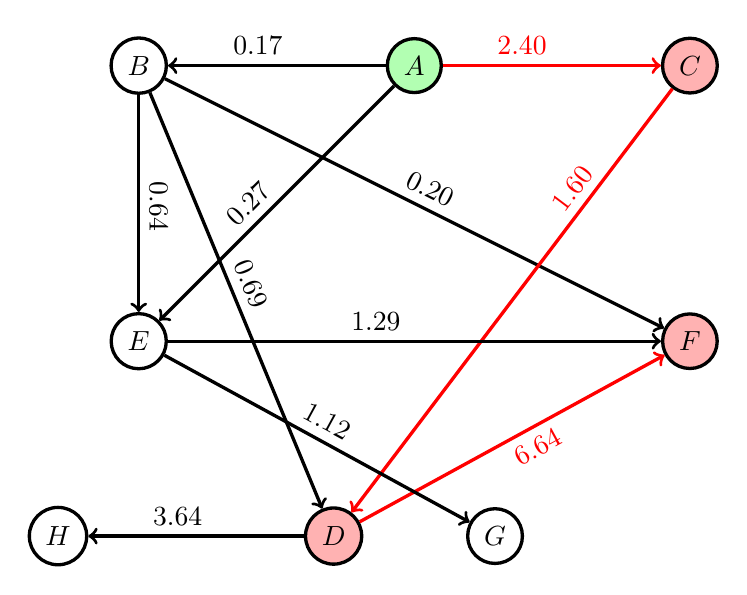
\begin{tikzpicture}[node distance={35mm}, very thick, main/.style = {draw, circle}] 

    \node[main, fill=green!30] (0) {$A$}; 
    \node[main] (1) [left of=0] {$B$}; 
    \node[main, fill=red!30] (2) [right of=0] {$C$};  
    \node[main] (4) [below of=1] {$E$}; 
    \node[main, fill=red!30] (3) [below right of=4] {$D$};
    \node[main, fill=red!30] (5) [below of=2] {$F$}; 
    \node[main] (6) [below left of=5] {$G$}; 
    \node[main] (7) [left of=3] {$H$};

    \draw[->] (0) -- node[midway, above right, sloped, pos=0.75] {0.17} (1);
    \draw[red,->] (0) -- node[midway, above right, sloped, pos=0.2] {2.40} (2);
    \draw[->] (0) -- node[midway, above right, sloped, pos=0.67] {0.27} (4);
    \draw[->] (1) -- node[midway, above right, sloped, pos=0.4] {0.69} (3);
    \draw[->] (1) -- node[midway, above right, sloped, pos=0.35] {0.64} (4);
    \draw[->] (1) -- node[midway, above right, sloped, pos=0.45] {0.20} (5);
    \draw[red,->] (2) -- node[midway, above right, sloped, pos=0.33] {1.60} (3);
    \draw[red,->] (3) -- node[midway, below right, sloped, pos=0.45] {6.64} (5);
    \draw[->] (3) -- node[midway, above right, sloped, pos=0.75] {3.64} (7);
    \draw[->] (4) -- node[midway, above right, sloped, pos=0.35] {1.29} (5);
    \draw[->] (4) -- node[midway, above right, sloped, pos=0.4] {1.12} (6);        

\end{tikzpicture}
\end{center}    
\end{figure}  

    
\newpage

\begin{figure}[ht]
\centering

%% Aposxoliaste tin epomeni grammi kai xrisimopoieiste to 
%% katallilo onoma arxeiou gia na pros8esete tin eikona sas
%\includegraphics[width=4cm]{img1.png}

% Create a plot
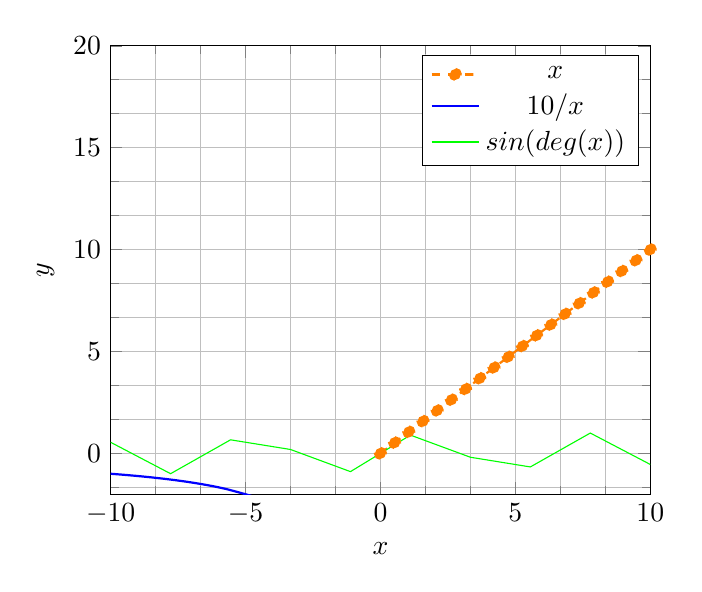
\begin{tikzpicture}
    \begin{axis}[xmin=-10, xmax=10, ymin=-2, ymax=20, grid=both, 
                major grid style = {lightgray},
                minor tick num = 2,
                minor grid style = {black!25},
                xlabel=$x$, ylabel=$y$]
        \addplot[domain=0:10, samples=20, smooth, thick, dashed, orange, mark=*]{x};
        \addplot[domain=-10:-1, samples=20, smooth, thick, blue]{10/x};
        \addplot[domain=-10:10, samples=10, green]{sin(deg(x))};
        \legend{$x$, $10/x$, $sin(deg(x))$}
    \end{axis}
\end{tikzpicture}

\caption{Γράφημα Άσκησης 5}
\label{my_graph_ask5}
\end{figure} 

\ldots όπως φαίνεται στο Σχήμα \ref{my_graph_ask5} \ldots


``τάξη'' στα ελληνικά και \en{``order''} στα αγγλικά

\begin{itemize}
    \item $\mathcal{O}(n!)$
    \item $O(n!)$
    \item $o(3^n)$
    \item $\Omega (\log n^c)$
    \item $\omega (\log n!)$
    \item $\omega (\log n!)$
    \item $\Theta (n)$
    \item $\sim$
    \item $\sqrt[3]{n^\alpha}$
    \item $x \in \mathbb{N}, \notin$
    \item $\exists, \nexists, \forall$
    \item $\Rightarrow$
    \item $\Leftrightarrow$
    \item $\leq, <, \geq, >$
    \item $\lim_{n\to\infty} n$
    \item $\sum_{i=0}^{\infty} i$
    \item $\frac{n+1}{n^2}$
\end{itemize}


\newpage

    % Use english
    \en{    

        % New algorithm
        \begin{algorithm}
            \begin{algorithmic}[1]
            \caption{}

                \Procedure{calc}{$w$}
                    \State $res \gets 0$
                    \For{$i \gets 1$ to $w^{0.5}$ with step 0.1}
                        \State $res \gets res + \log(i)$
                    \EndFor                    
                    \State \Return res
                \EndProcedure
                \\
                \State $arg \gets -1$

                \For{$i \gets 1$ to $2n$ with step 1}
                    \For{$j \gets i$ to $i^{2}$ with step 1}
                        \State $arg \gets CALC(j)$
                    \EndFor
                \EndFor
                
            \end{algorithmic}
        \end{algorithm}  
    }


\end{document}